\chapter{Integration of IO Channels in MIDG2}
\label{cha:sys_arch}

MIDG2\footnote{\url{https://github.com/tcew/MIDG2}} is used as the target
application in this thesis to evaluate the benefits of using IO channels.
MIDG2 application uses the \ac{DG} method to calculate the electric and magnetic
field values for objects as described in the chapter \todo{add chapter number}.
The thesis extends a version of the application which uses OpenCL™ kernels to
offload the performance critical calculations to the FPGA accelerators in a
distributed system and use MPI to communicate among the different instances of the
host application. The system scales over multiple nodes as discussed in section
\ref{sec:fpga_dg} but suffers from slow bandwidth due to the longer communication
path over PCIe and Ethernet Network of host. To improve the bandwidth performance
of the application, the IO channels are proposed to be used. This chapter will
introduce and explain the changes which were done to the OpenCL™ kernels and the
host application in order to use the QSFP Network Ports to build up topologies discussed
in chapter \ref{cha:topologies} to allow direct communication between the FPGAs
and reduce the communication time.

\section{Kernel Structure of MPI MIDG2 FPGA Implementation}
\label{sec:midge_mpi}

The MPI MIDG2 FPGA version requires an additional \texttt{partial\_get\_kernel} to gather the shared elements from
the main element buffer \texttt{g\_Q} into a smaller buffer partial data buffer \texttt{g\_partQ}.
The main benefit of using the additional kernel is to avoid the large memory transaction between the
host and the FPGA over PCIe to get the \texttt{g\_Q} and assemble the shared buffers in host.
The addition of the partial kernel was accompanied with resshuffling of the elements in the \texttt{g\_Q}
buffer. The distributed design requires the mesh to be partitioned into smaller meshes allocated
to each rank. The elements of the partitioned mesh can either share a face with a neighboring
rank or within the rank. The elements which share faces with neighboring ranks form the shared
element group and the ones sharing faces within rank form the non-shared element group.
To separate the computation of the these shared element group and the non-shared element group
by reusing the same kernels required sorting of the elements into groups. This was done by
placing the shared elements in the start of the \texttt{g\_Q} buffer followed by the shared
elements. This allowed to use the same kernels with different start and end element parameters
to be invoked for processing the shared and non-shared elements separately.


\TODO{add image to show the reaarangement to }

The original pipeline developed for single FPGA was further optimized by introducing separate buffers
\texttt{volrhsQ} and \texttt{surrhsQ} instead of the the same right hand side \texttt{rhsQ} buffer
which was earlier accumulated in surface kernel. These changes allows the volume and surface kernel
to execute parallely and write data into two separate buffers. The RK kernel reads both the buffers
after volume and surface kernel are finished processing and accumulates the values using rungga-kutta
constants to produce the field values for the timestep. Another improvement introduced to optimize the
design was to use the concept of double buffers for the \texttt{g\_Q}. The \texttt{g\_Q} buffer is
duplicated into two buffers \texttt{g\_Q\_ping} and \texttt{g\_Q\_pong} which use two alias \texttt{g\_Q\_in}
and \texttt{g\_Q\_out} in the kernel. The \texttt{g\_Q\_in} serves as the buffer from which the kernels read
the elements values for the current iteration wheres \texttt{g\_Q\_out} serves as buffer in which the values
are updated. After each time step iteration the alias of the buffers is switched as shown
in pseudo code in \ref{code:buff_switch}, exchanging the functionality of the buffers for the next iteration.

\begin{CppCode}[caption=Buffer switching for double buffers in each iteration, frame=tlrb, label=code:buff_switch]
for (itr = 0; itr < MaxTimeStep; itr++)
{
    if (buffSwitch)
    {
        set_argument("g_Q_in", Q1_pong_mem);
        set_argument("g_Q_out", Q1_ping_mem);
    }
    else
    {
        set_argument("g_Q_in", Q1_ping_mem);
        set_argument("g_Q_out", Q1_pong_mem);
    }
    buffSwitch = !buffSwitch;
}
\end{CppCode}

The concept helps to improve the performance of the RK kernel
by removing read and write memory dependency on the same buffer. In each time step,
the volume kernel and surface kernel first execute to compute the right hand side values for the
non-shared elements while the shared data is exchanged. Once the shared data is available,
the right hand side values for the shared elements is computed. After the computation,
the RK kernels reads the field values from \texttt{g\_Q\_in} and \texttt{resQ} values
for the last time steps and computes the accumulated field values using
\texttt{volrhsQ} and \texttt{surrhsQ}. The computed values are then saved in \texttt{g\_Q\_out}.
As the read and write buffers are separated, the memory dependency on the same buffer is reduced,
reducing the latency to read and write to the memory. As explained, this structure also allows
to overlap the communication via MPI with the computation of the fields for the non-shared data
and reducing the effects of delayed communication. The kernel structure for base MPI MIDG2 FPGA
is shown in Figure \ref{fig:base_kernstruc}.

\begin{figure}%
    \centering
    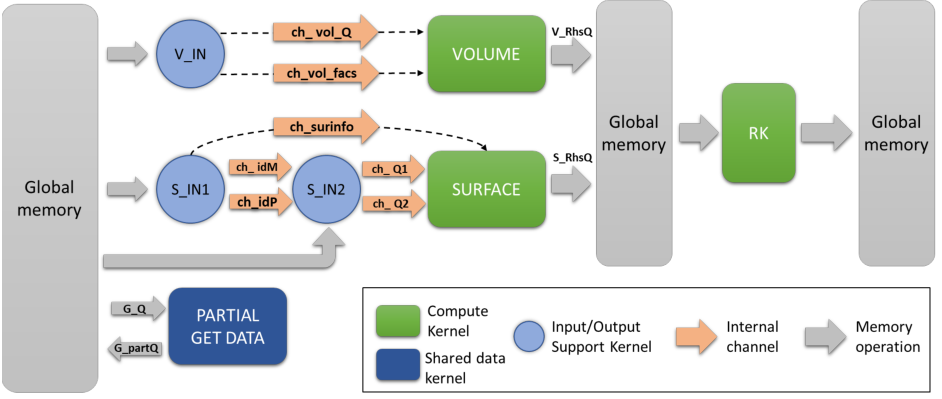
\includegraphics[width=1.0\textwidth]{images/base_kernstruc}
    \caption{Structure for MPI FPGA OpenCL™ kernels showing the partial get kernel used to gather
     the shared elements into a separate buffer \texttt{g\_partQ} for host to read}
    \label{fig:base_kernstruc}
\end{figure}

\section{Kernel Structure with IO Channels}
\label{sec:struc_iochan}

The prototypes developed for the topologies evaluation served as the basis to implement
the support for IO channels in the OpenCL™ kernels for the MIDG2 application. The main
modification required to enable the OpenCL™ MIDG2 kernels to communicate via IO channels
was to remove the \texttt{partial\_get\_kernel} and replace with two kernels
\texttt{partial\_send} and \texttt{partial\_recv}. The implementation of these kernels
is similar to the prototype \texttt{send} and \texttt{recv} kernels described in
section \ref{sec:proto_topo}. Two different set of kernels for the two topologies,
the within node using 2 FPGAs on the same node and fully connect topology using
4 FPGAs on two nodes was developed.

\TODO{explain the channels implementation further with source code to highlight that,
aliasing of the g\_partQ buffer for fully connect design}

\begin{figure}%
    \centering
    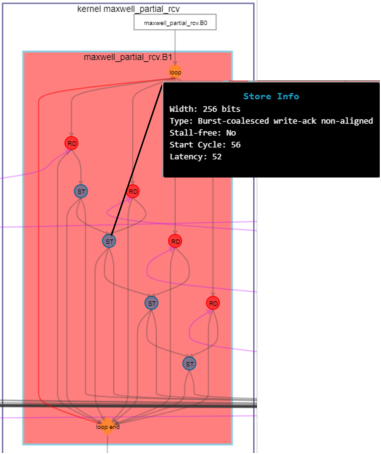
\includegraphics[width=0.5\textwidth]{images/serial_reads}
    \caption{Memory dependency resulting in serial channel reads in the \texttt{partial\_recv}
    for fully connected design}
    \label{fig:serial_reads}
\end{figure}


An additional optimization to kernel pipeline
was also introduced which helps to improve the performance of the kernels marginally.
Intel® OpenCL™ channels are used to communicate the right hand side field values
from volume and surface kernels to the RK kernel as shown in the kernel structure
in figure \ref{fig:iochan_kernstruc}. Use of channels allows execution of all three
kernels simultaneously giving a deeper pipeline structure and improving the throughput
of the design by performing parallel computation in volume, surface and RK kernels.

\begin{figure}[h]%
    \centering
    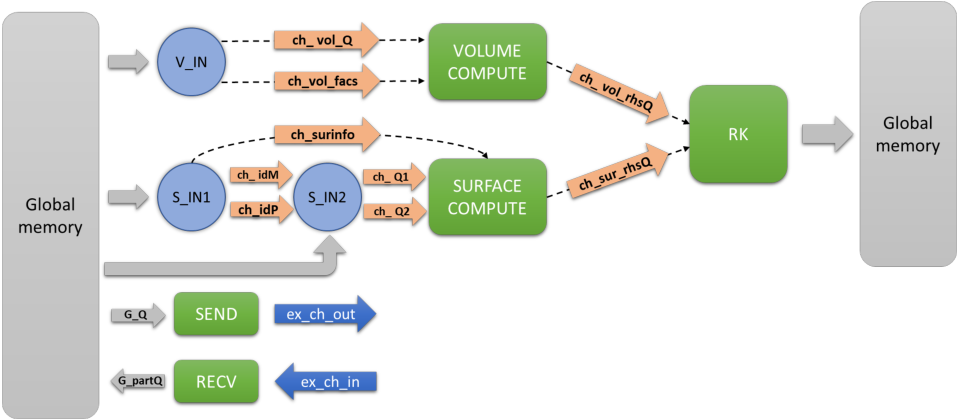
\includegraphics[width=1.0\textwidth]{images/iochan_kernstruc}
    \caption{Structure for MPI FPGA OpenCL™ kernels showing \texttt{send} and \texttt{recv}
    kernels used for communication with external IO channels. Image also shows the internal
    channels introduced between volume/surface to rk kernel}
    \label{fig:iochan_kernstruc}
\end{figure}

As in the MPI MIDG2 FPGA design, the computation of shared elements follows the computation of
non-shared elements. The major change is the independence of the OpenCL™ kernels to
communicate the data between the FPGAs without requiring support of the host for
communication. Though host still controls the time step iteration and performs synchronization of kernels between
the computation of non-shared data and the completion of communication of data between two FPGAs.
A comparison of the sequence of operations performed on host and FPGA for the MPI MIDG2 FPGA and
the IO channels design is shown in figure. As the figure shows, the involvement of the host is
decreased. Also due to addition of the channels between the volume/surface and RK kernel,
all kernels in the new design start together instead of RK following volume/surface.

\begin{figure}[h]
	\centering\small
	\begin{tabular}{l@{\hskip 0.5in}}
        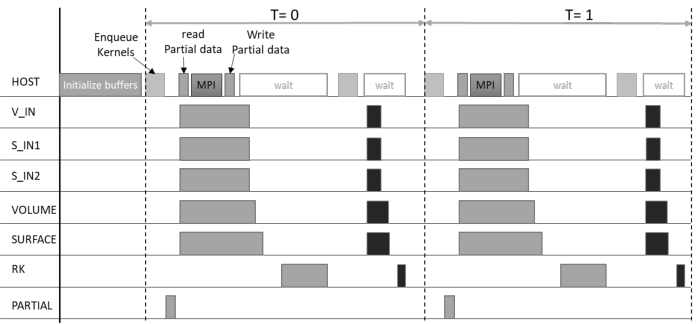
\includegraphics[width=0.8\textwidth]{seq_singlefpga} \\
        \multicolumn{1}{c}{(a) MPI MIDG2 FPGA}  \\
        \\
        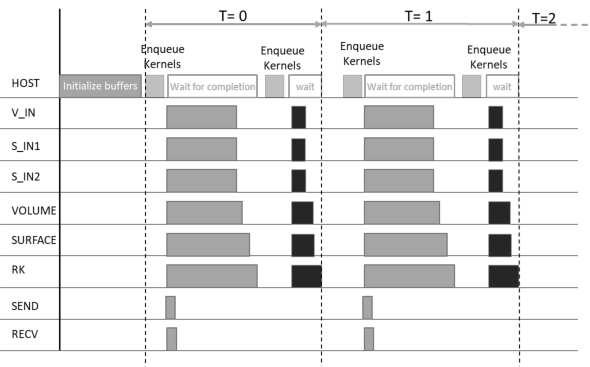
\includegraphics[width=0.7\textwidth]{seq_iochan} \\
        \multicolumn{1}{c}{(b) MIDG2 FPGA with IO channels}
	\end{tabular}
    \caption{Sequence of Kernel and host event for MPI MIDG2 FPGA
    and MIDG2 FPGA with IO channels}
	\label{fig:topologies}
\end{figure}

\section{Host changes for to support IO Channels}

The host MIDG2 implements the 3D DG-method introduced in the section \ref{sec:dgtd}.
The application is responsible for following activities:

\begin{itemize}
    \item Read in the mesh and parse the element coordinates and save them in VX, VY and VZ vectors
    \item For a distributed implementation using MPI, partition the mesh using parMETIS library
    and redistribute the elements as per the partition.
    \item Create the information of the shared elements which should be used to identify and map the
    indexes in the field buffer to be shared with the target MPI ranks. The mapping is used to read the
    values and create the partial data buffers to be communicated via MPI or FPGA-to-FPGA link
    \item Perform polynomial interpolation mapping of the geometric element vectors to the standard tetrahedral
    element coordinates using r, s and t values
    \item Compute the geometric coefficients and data layout information (\texttt{vmapM} and \texttt{vmapP})
    \item Setup the OpenCL™ environment which includes identifying the OpenCL™ platform and device,
    create OpenCL™ memory buffers to be used, copy the data to OpenCL™ memory buffers, program the FPGA with the
    target OpenCL™ kernel binary and create OpenCL™ queue to run the kernels.
    \item Run the OpenCL™ kernels and synchronize the execution over the computed timesteps
    \item Read the results value and compare the analytical and computed results to compute the error
    to estimate the accuracy of the implementation
\end{itemize}

The changes in the host application done mainly are towards enabling the new kernels to function correctly
which involves setting up the OpenCL™ buffers and control the queueing of the kernels in the correct sequence.
To handle this, the structure of the existing OpenCL™ initialization code sections is updated to handle
both the designs with the same host code. A hierarchical structure for the OpenCL™ initialization code
is implemented such that, the generic functionalities which is separated from the design specific buffer
initialization and kernel enqueue sequence setup. The new structure of the host code is shown
in figure \todo{add image of the host code structure} and would be explained in the section ref{sec:hostcodeupdate}.

The host application requires an additional json file to get the information about the kernels in the binary such as
the kernel parameter information, dependencies among the kernels and groups of kernels to be executed parallely.
These information is used to configure the kernel buffers as well as setup a execution order tree which is used
to enqueue the kernels in required order and setup other kernel to kernel synchronization using the events.
The main benefit of using the configuration json file is to ease the setup effort for the dependent kernel.
The subgroup structure of the kernels in IO channels design is shown in listing \ref{code:subgroups}.

\begin{JsonCode}[caption=Kernel subgroups used in Multi FPGA design to enqueue kernels, frame=tlrb, label=code:subgroups]
"kernel_subgroups":
{
    "compute_inner":
    {
        "single_work_item": "true",
        "kernels":
        {
            "maxwell_partial_send":{},
            "maxwell_partial_rcv": {},
            "inputkernel_vol": {},
            "maxwellvolumekernel": {},
            "inputkernel": {},
            "maxwellsurfacekernel": {},
            "inputkernel1": {},
            "maxwellrkkernel": {}
        }
    },
    "compute_halo":
    {
        "single_work_item": "true",
        "kernels":
        {
            "inputkernel_vol": {},
            "maxwellvolumekernel": {},
            "inputkernel": {},
            "maxwellsurfacekernel": {},
            "inputkernel1": {},
            "maxwellrkkernel": {}
        }
    }
}
\end{JsonCode}

The \texttt{compute\_inner} subgroup is responsible for computing the field values for the non-shared
data and perform the data exchange between the FPGAs using the IO channels. As there is no dependencies
listed among any of the kernels in the subgroup, each of the kernels will be executed simultaneously.
The \texttt{compute\_halo} subgroup performs the computation on the shared elements. As the same kernels
are responsible for performing the computation on the shared and non-shared elements, the kernels are
repeated in both the groups. The subgroups help to easily create a execution tree grouping
the same kernels in different groups and order depending upon the implementation which can then be
easily executed on the FPGA device.

Another important modification is done in the host application to get the information about
the mapping of the MPI ranks to the FPGA devices on the node. This mapping is required for the
fully connect topology to setup the correct offsets and number of elements for each of the channels.
The mapping information allows to associate a specific external channel with a MPI rank and hence the
offsets within the \texttt{g\_index} buffer which contains the index values in the \texttt{g\_Q}
buffer for the shared elements. To map the channels, additional information
regarding the MPI rank and associated FPGA device is required. This information is shared using
a structure which contains the MPI host id and associated FPGA device Id which is exchanged
using MPI. After receiving the information about all the ranks, the external channel mapping
is computed locally using a decision tree. The flow chart in figure \todo{add flowchart to explain the selection}
shows the logic of the external channel assignment at each node.

